\newpage
\section{Particle characterization and particle tracking using holographic video microscopy}
		\label{sec:chapter2}

\subsection{Introduction}

Properties of coherent light to produce interference is widely used in metrology for a long time with the famous Fabry-Pérot  \cite{fabry_theorie_1899, perot_application_1899} or Michelson interferometer \cite{michelson_relative_1887} which was initially used to measure the earth rotation and is still used today, in particular, for the recent measurement of gravitational waves
\cite{ligo_scientific_collaboration_and_virgo_collaboration_gw151226_2016}. 
Since the beginning of the century, interest on tracking and characterizing colloidal particles risen thanks to the democratization of micro fluidics and lab-on-a-chip technologies. A lot of methods were developed, I will in the folowing give some insights on the three most used :

\begin{itemize}
	\item Reflection Interference Contrast Microscopy (\gls{RICM})
	\item Lorenz-Mie fit
	\item Rayleigh-Sommerfeld back-propagation
\end{itemize}

Experimentaly, this methods are generaly implemented in setups where the the incident light and scattered (or reflected) ligth are colinear, we thus speak of in-line holography.

\subsection{In-line holographic video microscopy theory}

\subsubsection{Reflection Interference Contrast Microscopy}

\begin{figure}[h]
	\centering
	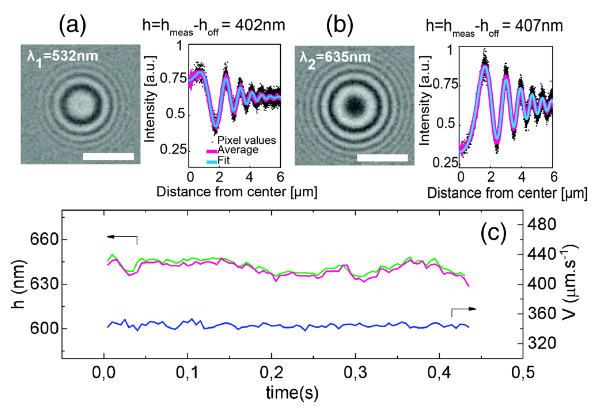
\includegraphics[scale=0.8]{02_body/chapter2/images/RICM.png}
	\caption{Figure from \cite{davies_elastohydrodynamic_2018} representing \gls{RICM} with two wavelength. (a) Left: interference patterns created with a wavelength $\lambda_1 = 532$ nm (scale bar $ 5~\mathrm{\mu m}$). 
		Right: radial intensity profile (black dots) extracted from the image, azimuthally averaged (magenta line) and fitted with Eq.\ref{Eq.RICM} to measure the height of the particle here donated with ($h$). (b) Same as (a) with a wavelength $\lambda_2 = 635$ nm. (c) Time series of the height of the particle $h$ (green: $ \lambda_1$, magenta: $\lambda_2$) and the particle velocity along the flow in blue. }
	\label{fig.RICM}
\end{figure}


Reflection Interference Contrast Microscopy was first introduced in cell biology by Curtis to study embryonic chick heart fibroblast \cite{curtis_mechanism_1964} in 1964. \gls{RICM} gained in popularity 40 years after both in biology and physics \cite{filler_reflection_2000, siver_use_2000, weber_2_2003, limozin_quantitative_2009, nadal_probing_2002, raedler_measurement_1992}. It was also used recently in soft matter physics to study elastohydrodynamic lift at a soft wall \cite{davies_elastohydrodynamic_2018}.

When we illuminate a colloid with a plane wave, a part of the light is reflected from the surface and interference fringes appear. Let's take an interest at the mathematical description of this phenomenon. In the far field, we can describe two different one-dimensional electric field vectors of the same pulsation $\omega$ \cite{f_bohren_absorption_1998} as:

\begin{equation}
	\vec{E_1}(\vec{r}, t) = \vec{E_{0_1}} \cos(\vec{k_1} \cdot \vec{r} - \omega t + \epsilon_1) ~,
\end{equation}
and
\begin{equation}
	\vec{E_2}(\vec{r}, t) = \vec{E_{0_2}} \cos (\vec{k_2} \cdot \vec{r} - \omega t + \epsilon_2) ~.
\end{equation}


\nomenclature{$\vec{E}$}{Electrical field}
\nomenclature{$k$}{Wave number}
\nomenclature{$\omega$}{Pulsation}

Where the $k$ is the wave number $k=2\pi n_{solvent}/\lambda$, $\lambda$ denoting the wavelength, $n_solvent$ the optical index of the solvent, $\epsilon_{1,2}$ the initial phase of each waves and $\vec{r}$ the position from the source, here, it is the distance between the glass slides where happens the first relflection and the particle. The intensity we observe can be computed from the time averaged of the squared sum of the eletric field $\vec{E} = \vec{E}_1 + \vec{E}_2$. The measured intensity is thus given by:

\begin{equation}
	\begin{aligned}
		I & = \langle \vec{E}^2 \rangle = \langle \vec{E}_1^2 + \vec{E}_2^2 + 2\vec{E}_1 \cdot \vec{E}_2 \rangle 
		= \langle \vec{E}_1^2 \rangle + \langle \vec{E}_2^2 \rangle  + 2 \langle \vec{E}_1 \cdot \vec{E}_2 \rangle \\
		& = \frac{{E_{0_1}^2}}{2} + \frac{{E_{0_2}^2}}{2} +  2 \langle \vec{E}_1 \cdot \vec{E}_2 \rangle ~,
	\end{aligned}
\end{equation} 

where $ \langle \vec{E_1} \rangle $ and  $\langle \vec{E_2} \rangle$ are respectively given by $I_1$ and $I_2$. Using the trigonometric formula $2 \cos (a)\cos (b) = \cos (a+b) \cos (a-b) $ we have:

\begin{equation}
	\langle  
	\vec{E}_1 \cdot \vec{E}_2 \rangle = 
	\langle
	\frac{1}{2} \vec{E}_{0_1}  \vec{E}_{0_2} 
	\left[
		\cos 
		\left(
			\vec{k}_1 \cdot \vec{r} - \vec{k}_1 \cdot \vec{r} + \phi	
		\right)	
		+ 
		\cos
		\left(
			2\omega t + \phi'
		\right)
	\right]
	\rangle~.
\end{equation}

As we average over the time, the second $\cos$ will vanish since in general $\langle \cos(at + b) \rangle_ t = 0$ thus:

\begin{equation}
	\langle \vec{E}_1 \cdot \vec{E}_2 \rangle = \frac{1}{2} \langle  \vec{E}_{0_1}  \vec{E}_{0_2} \rangle
	\cos 
	\left(
	\vec{k}_1 \cdot \vec{r} - \vec{k}_2 \cdot \vec{r} + \phi	
	\right)	
\end{equation}

with $\phi$ the phase difference between the two fields, which is generaly equal to $\pi$ due to the reflection properties.  finaly, the total intensity can be read as:


\begin{equation}
	I = I_1 + I_2 + 2 \sqrt{I_1 I_2} 
	\cos 
	\left(
	\vec{k}_1 \cdot \vec{r} - \vec{k}_2 \cdot \vec{r} + \phi	
	\right)
\end{equation}

If the indicent and reflected wave are parallel we can work in 1 dimension and we have $k_1 = - k_2$ and simplifying $\vec{r}$ to simply $z$ the height of the particle we have:


\begin{equation}
	I = I_1 + I_2 + 2 \sqrt{I_1 I_2} 
	\cos 
	\left(
	\frac{4 \pi n_{solvent}}{\lambda} z + \phi	
	\right)
\end{equation}


If we now suppose that we have a spherical particle at a height $z$ we can write the radial interference intensity $I(x)$ as \cite{ raedler_measurement_1992}:

\begin{equation}
	I(x) = A_0 + A_1 \mathrm{e}^{-b_1 x^2} + A_2^{-b_2 x^2} \cos \left[ \frac{4\pi n_m}{\lambda}\left( g(x) + z \right) + \phi \right]
	\label{Eq.RICM}
\end{equation}

Where $A_i$ and $b_i$ are fit parameters and $g(x)$ donotes the contour of the sphere.
Finally, this method is great because the equation are computationaly light and permits to have a quick tracking of particles. However, as we can see on Eq.\ref{Eq.RICM} the interference pattern will be the same for all heights $z$ separated by a distance $\lambda / 2n \approx 200 $ nm for typicaly used light in water ($\lambda = 532$ nm and $n_{solvent} = 1.33$). It is possible to extend this limitation by using 2 differents wavelength to $\approx 1.2 ~ \mathrm{\mu m}$ as used in \cite{davies_elastohydrodynamic_2018}. Also, the small particle ($<5 ~ \mathrm{\mu m}$) will scatter to much compared to the reflection and the method will not work properly.  Despite the effectiveness of this method which can reach the $10$ nm precision on the particle position measurement, the range limitation are not compatible with the study of $ 1 ~ \mathrm{\mu m}$ particle's Brownian motion making \gls{RICM} not usable for our context.



\subsubsection{Lorenz-Mie Fit}

Another method to create hologram, is to look at the superimposition of the scatterd field $\vec{E}_s$ and incident field $\vec{E}_0$. This way, we could track and characterize even small particles. This method is has been developed in the early 2000 \cite{ovryn_imaging_2000, lee_characterizing_2007}. Since, a lot of studies has been realised with this method[cite a bunch of paper here]. 

Let's the incident field be a plane wave uniformly polarized along the axis $ \hat{e}$, with an amplitude $E_0$ and propagating along the $z$ direction :
\begin{equation}
	\vec{E}_0(\vec{r},z) = E_0(\vec{r}) \mathrm{e}^{ikz}\hat{e}
\end{equation}

Let's consider a particle of radius $a$ at a position $\vec{r}_p $, the scattered field can be written using the Lorenz-Mie theory \cite{f_bohren_absorption_1998} as:

\begin{equation}
	\vec{E}_s(\vec{r}) =  f_s(k(\vec{r} - \vec{r}_p))E_0(\vec{r}) \exp \left(-ikz\right) 
\end{equation} 

With $f_s$ the Lorenz-Mie scattering function \cite{f_bohren_absorption_1998}. The intensity $I$ that we measure at $\vec{r}$ is given by the super imposition of incident and scattered waves. Since the measurements are done at the focal plane, $I$ is given by:

\begin{equation}
	\begin{aligned}
	I(\vec{r}) & = |\vec{E}_s(\vec{r}, 0) + \vec{E}_0(\vec{r}, 0)|^2 \\
	& = E_0^2(\vec{r}) + 2 E_0^2\operatorname{Re} \left(f_s(k(\vec{r}- \vec{r}_p)) \hat{e}\right) + | f_s(k(\vec{r}- \vec{r}_p)) |^2
	\end{aligned}
\end{equation}

The most of the experimental defects on the images are due to spacial illumination variation caused by dust particle and such. It can be corrected by normalizing the image by the background. In another word, we normalize  $I(\vec{r})$ by the intensity of the incident field $E_0(\vec{r})^2$ which is the experimental background. It can be measured by different methods, one is to have an empty field of view and the other one, which is more convenient is to take the median of a stack of images. The latter also permits to get rid of the immobile particle that could generate any additional noise. An example of an hologram before and after the normalization is shown in Fig.XXX. We write the normalized intensity $b(\vec{r})$:

\begin{equation}
	b(\vec{r}) = 1 + 2 \operatorname{Re} 
	\left(  
		f_s(k(\vec{r}- \vec{r}_p)) \hat{e}
	\right)
	+
	|
		f_s(k(\vec{r}- \vec{r}_p))
	|^2
	\label{Eq.normalized_Mie}	
\end{equation}


Now that we have the analytical form of the holograms intensity it is possible to fit an experimental one to Eq.\ref{Eq.normalized_Mie} as shown in Fig.XXX. For the sake of completeness I will detail the Lorenz-Mie scattering function, $f_s(k\vec{r})$, it is given by the series:

\begin{equation}
	f_s(k \vec{r}) = \sum _{n=1} ^{n_c} 
	\frac
	{
		i^n (2n +1)
	}
	{
		n(n+1)
	}
	\left(
		i a_n \vec{N}^{(3)}_{eln}(k\vec{r})
		-
		b_n \vec{M}^{(3)}_{oln}(k\vec{r})
	\right)
	\label{Eq.Lorenz-Mie-function}
\end{equation} 


where $\vec{N}^{(3)}_{eln}(k\vec{r})$ and $\vec{M}^{(3)}_{oln}(k\vec{r})$ are the vector spherical harmonics. $a_n$ and $b_n$ are some coefficients that depend on the particle properties and illumination properties. For a spherical and isotropic particle of radius $a$ and refractive index $n_p$ which is illuminated by a linearly polarized plane wave, the coefficients are expressed in terms of spherical Bessel $j_n$ and Hankel $h_n$ functions as \cite{f_bohren_absorption_1998}:

\begin{equation}
	a_n = 
	\frac
	{
		\zeta^2 j_n (\zeta k a)k a j_n' (k a) - j_n(ka)[\zeta kaj_n(\zeta ka)]'
	}
	{
		\zeta^2 j_n (\zeta k a)k a h_n^{(1)'} (k a) - h_n^{(1)}(ka)\zeta kaj_n'(\zeta ka)
	}
\end{equation}

and

\begin{equation}
	b_n =
	\frac
	{
		j_n(\zeta k a) kaj_n'(ka) - j_n (ka) \zeta kaj_n'(mka)
	}
	{
		j_n(\zeta k a) kah_n^{(1)'}(ka) - h_n^{(1)} (ka) \zeta kaj_n '(mka)
	} ~,
\end{equation}


where $\zeta = n_p / n_m$ while the prime notation denotes differentiation with respect to the argument. As we can see, the holograms given by Eq.\ref{Eq.Lorenz-Mie-function} will vary with a lot of parameters ($\lambda$, $n_m$, $n_p$, $a$ and $r_p$) which can all be fitted. In general, the illumination wavelength and medium index are known and we are able to fully characterize a unique particle as well as precisely measure it's position. It is even possible to characterize a particle without a priori knowledge of it's characteristics using Bayesian approach \cite{gregory_bayesian_2005, dimiduk_bayesian_2016}.

 Another interesting question here, is until which number of terms the series Eq.\ref{Eq.Lorenz-Mie-function} converge. It has been found \cite{lentz_generating_1976} that the series converge after a number of terms
\begin{equation}
	n_c = k a + 4.05 (k a)^{1/3} + 2 ~.
\end{equation}
Thus, larger particles will need more time to be tracked. As an exemple, the largest particle used during my thesis have a radius $a = 2.5 ~ \mathrm{\mu m}$ leading to a number of terms $ n_c = 55$ in water and $\lambda = 532$ nm, for the smallest $a = 0.5 ~ \mathrm{\mu m}$ we find $n_c = 18$ which makes a huge difference in practice.

Finally, Lorenz-Mie is the most versatile in-line holographic method as it permits to track and characterize unique particles even without a priori knowledge. Besides, writing the $f_s$ function for particular particles such as anisotropic \cite{fung_holographic_2013}, non-spherical \cite{wang_using_2014} or clusters \cite{fung_holographic_2013, perry_real-space_2013} of particles permits to use this fitting method in more complex situations . Also it can reach really high precision as the tenth of nanometer on the position and radius and $10^{-3}$ on the optical index \cite{lee_characterizing_2007}. Unfortunately, the Lorenz-Mie fitting suffer from a major drawback which is the time needed to fit one image. For example, a 200 by 200 pixels image of a $2.5 ~ \mathrm{\mu m}$ particle's hologram can take up to 2 seconds to be fitted using a pure python algorithm. A lot of work as been done to have faster tracking such as random-subset fitting \cite{dimiduk_random-subset_2014}, GPU (graphical processing unit) acceleration, machine-learning \cite{yevick_machine-learning_2014, hannel_machine-learning_2018} and deep neural networks \cite{altman_catch_2020}.

\subsubsection{Reyleigh-Sommerfeld back propagation}
Bon faut s'attaquer au R-SBP un jour :((

\subsection{Experimental setup}
J'explique ici le setup experimental et comment il faut bien choisir son objectif en side note !!

\subsection{Numerical treatment ??}

Ici je vais présenter comment j'inverse les holograme, je vais présenter holopy et le code de groupe de grier. Expliquer aussi les limitations temporelles et comment j'ai essayer de les contourner pour finalement dire qu'un doctorant de chez grier a fini de dévelloper l'accélération GPU qui a rendu l'inverversage des trajectoire a un temps humain !

\subsection{Radius and optical index characterization}


Ici je vais présenter la characterization et les graphs de n en fonction de r et de discuter la dépendence apparente de r/n où je vais certainement m'appuyer sur un des papiers de Grier. 

